\documentclass[[12pt,conference]{IEEEtran}
\IEEEoverridecommandlockouts
% The preceding line is only needed to identify funding in the first footnote. If that is unneeded, please comment it out.
\usepackage{cite}
\usepackage{pgfplots}
\pgfplotsset{width=7cm,compat=1.8}
\usepackage{amsmath,amssymb,amsfonts}
\usepackage{algorithmic}
\usepackage{graphicx}
\usepackage{textcomp}
\usepackage{xcolor}
\usepackage{layouts}
\usepackage{float}
\usepackage{listings}
\usepackage{multirow}
\usepackage{hyperref}
\usepackage{subfig}


    
\usepackage{minted}
\RecustomVerbatimEnvironment{Verbatim}{BVerbatim}{}


\begin{document}

\lstdefinestyle{mystyle}{
    keywordstyle=\color{magenta},
    basicstyle=\ttfamily\footnotesize,
    breakatwhitespace=false,         
    breaklines=true,                 
    captionpos=b,                    
    keepspaces=true,                 
    numbersep=2pt,                  
    showspaces=false,                
    showstringspaces=false,
    showtabs=false,                   
    tabsize=2
}
\lstset{style=mystyle}


\title{\huge Predicting Fair Prices for HDB Resale Flats \\ \LARGE EE4802 Assignment 1 Report }

\author{\IEEEauthorblockN{Josiah Mendes}
\IEEEauthorblockA{\textit{National University of Singapore} \\
\textit{A0261318J} E0978323@u.nus.edu}\vspace{-3em}}

\maketitle

\section{Introduction}
This report presents the process of designing a regression model to predict fair prices for the resale of public housing flats in Singapore based on historical data obtained between Jan 1990 and Feb 2023.


\section{Data Information}
The latest historical data was obtained from \href{https://data.gov.sg/dataset/resale-flat-prices}{official government data} published by the Housing and Development Board on the 18th of February, 2023. 
The dataset comprises:
\begin{enumerate}
    \item Resale flat prices based on the approval date from Jan 1990 to Dec 1999 (287,196 records)
    \item Resale flat prices based on the approval date from Jan 2000 to Feb 2012 (369,651 records)
    \item Resale flat prices based on registration date from Mar 2012 to Dec 2014 (52,203 records)
    \item Resale flat prices based on registration date from Jan 2015 to Dec 2016 (37,153 records)
    \item Resale flat prices based on registration date from Jan 2017 to Feb 2023 (146,965 records)
\end{enumerate}

with a total of 893,168 records. 

The dataset does differ as pre-March 2012 transactions were dated by approval date while later transactions are dated by registration date, but as the difference between the two dates is usually within a month and hence unlikely to affect transaction prices, they are combined and treated as a single category. 

Each file contains the following attributes for each resale transaction:
\begin{table}[H]
\vspace{-1em}
\caption{Data Attributes}
\label{tab:data-attributes}
\centering
\begin{tabular}{c|c|c}
No. & Name                    & Type               \\ \hline
1   & Month                   & DateTime (YYYY-MM) \\
2   & Town                    & Categorical Text   \\
3   & Flat Type               & Categorical Text   \\
4   & Block                   & Text   \\
5   & Street Name             & Text   \\
6   & Storey Range            & Categorical Text   \\
7   & Flat Area               & Numeric (sqm)      \\
8   & Flat Model              & Categorical Text   \\
9   & Lease Commencement Date & DateTime (YYYY)    \\
10  & Remaining Lease         & Text (YY-MM)               \\
11  & Resale Price            & Numeric (SGD)     
\end{tabular}
\end{table}

Attribute 10 is only present on data from January 2015 onwards, but as it is just a re-expression of attribute 9 (all HDB flats in Singapore have a 99-year lease), it can be inferred for the other transactions with a reduced unit of precision due to Attribute 9 only having the year for the lease commencement date. This decision may have a slight impact on prediction accuracy if lease length is highly weighted by the model. 

As all the other data attributes are present in every subset of data, the CSV files were merged into a single file to facilitate easier data processing. 

\section{Data Cleaning}


\subsection{Removal of Redeveloped HDB Blocks}
The Selective En Bloc Redevelopment Scheme (SERS) is a government project that redevelops flats in older housing estates, demolishing old blocks and building new blocks. 
As the dataset includes transactions pertaining to demolished blocks that can share very similar attributes to existing blocks, these datapoints can lead to a decrease in prediction accuracy and can be considered outliers. 
Additionally, transactions for a flat in a soon-to-be demolished block may skew resale prices.
Therefore, as part of the cleaning process, all transactions that have been demolished under the scheme (obtained from \href{https://www.hdb.gov.sg/residential/living-in-an-hdb-flat/sers-and-upgrading-programmes/sers/sers-projects/completed-sers-projects}{HDB Published Completed SERS Projects}) are removed. 

One such example is the estates in Lim Chu Kang town which only had 64 resale transactions, further research showed that this estate was bought en-bloc by the Singaporean government in 2002. 
Therefore, as no further resale transactions can happen in that town and may skew other predictions due to the small sample size, it is removed.

All of the removed transactions are pre-2011 (the year the last completed SERS project happened), with more recent years of data unaffected, leaving 878,934 transactions. 
The amount of transactions removed (14,234) is relatively small compared to the size of the total dataset (1.59\%).
As there are still SERS projects ongoing, and future unannounced SERS projects, some of the data used for training will become ``invalid'' as time goes by. 

The combined data file with the SERS-affected transactions removed is used as the dataset before other pre-processing and feature engineering. (Uploaded as \texttt{resale-flat-prices-sers-removed.csv})

\subsection{Inconsistent Categorisation Correction}

\subsubsection{Flat Type}
The flat type category was noted during inspection to be inconsistent in its labelling of multi generation type flats, with some records using \texttt{Multi Generation} and others using \texttt{Multi-Generation}. 
These two categories were combined into a single category.

\subsubsection{Flat Model}
A similar phenomenon was noticed across multiple categories within Attribute 8, the flat model column with inconsistencies in spacing and capitalisation of category names. These were individually corrected, reducing the number of labels from 34 to 21. 


\section{Data Preprocessing}

% \subsection{Transaction Month} This attribute is transformed from the format \texttt{YYYY-MM} to the number of months since Jan 1990 to simplify the representation e.g (01-2023 $\to$ 384).

\subsection{Remaining Lease}
This attribute can be added to the dataset for all transactions by adding 99 years to the lease start date and subtracting the transaction year. 
The \texttt{lease\_commencement\_date} attribute is then dropped. 

\subsection{Categorical Data Transformation}
\subsubsection{Flat Type}
This attribute is primarily determined by the number of bedrooms + living rooms, ranging from 1 to 5. There are two additional types \texttt{Executive} and \texttt{Multi-Generation} which both have a mean larger square area. As there is a meaningful order, this data is transformed using an ordinal encoding ranging from 1 to 7. 

\subsubsection{Flat Model}
This attribute provides further insight into the flat design and features, with 21 unique values. The variance across the different types is high, indicating that this could be a key feature in regression. This attribute has no set order, so it is transformed using one-hot encoding. 

\subsubsection{Town}
This attribute describes which estate the flat is located in with 27 unique locations. As there is no meaningful relationship, the same one-hot encoding is applied. 

\subsubsection{Storey Range}
This attribute describes the range of storeys that a flat resale falls into, such as \texttt{10 TO 12} or \texttt{01 TO 03}. This categorical attribute is replaced by converting the range to the median value (e.g. \texttt{10 TO 12} $\to 11$).

\section{Feature Engineering}
\subsection{Transaction Month \& Resale Price}
Initial correlation studies showed that the transaction month category had the strongest correlation with the resale price (0.65). While this is true, essentially modelling house price inflation, it would not make sense for this to be the main attribute used for predictions at the current time. 

Another set of relevant data that is published is the \href{https://data.gov.sg/dataset/hdb-resale-price-index?view_id=14c47d07-1395-4661-8466-728abce27f5f&resource_id=52e93430-01b7-4de0-80df-bc83d0afed40}{HDB Resale Price Index} which tracks the overall price movement of the public residential market. This data can be used to normalise the resale price to provide an inflation-adjusted value. This adjustment increases correlation for expected attributes such as floor area, flat type and remaining lease (Fig \ref{Figure:FeatureCorrelationComparison}).

\begin{figure}[H]
  \centering
  \subfloat[Original Resale Price]{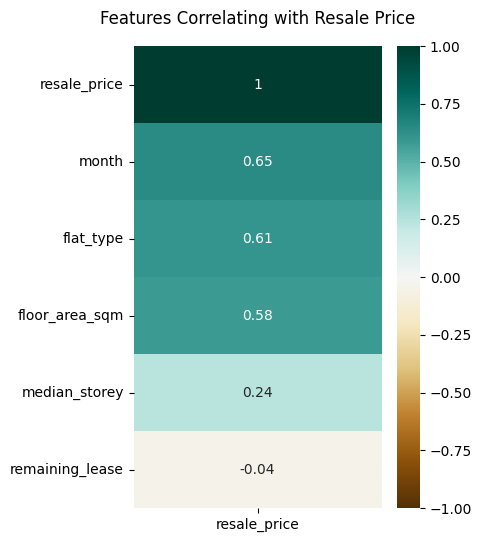
\includegraphics[width=0.45\linewidth]{resale_price_corr.png}\label{fig:f1}}
  \hfill
  \subfloat[Inflation-Adjusted Resale Price]{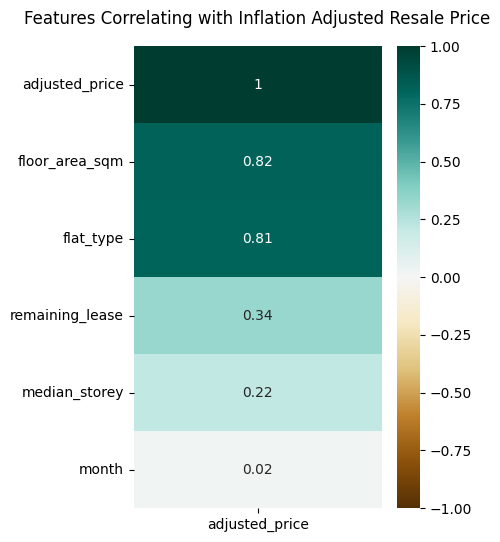
\includegraphics[width=0.45\linewidth]{resale_price_corr_inflation.png}\label{fig:f2}}
  \caption{Feature Correlation Comparison}
  \label{Figure:FeatureCorrelationComparison}
\end{figure}

\begin{figure}[H]
    \centering
    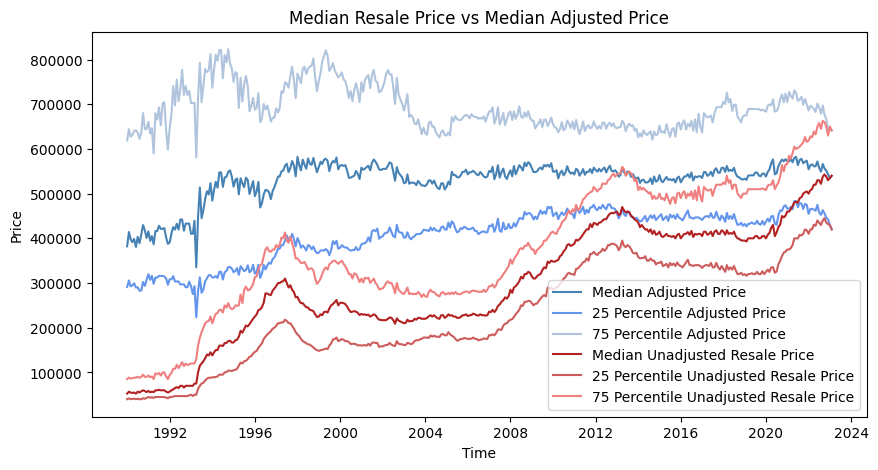
\includegraphics[width=\linewidth]{image.png}
    \caption{Inflation-Adjusted and Unadjusted Resale Price}
    \label{fig:price_adjustment}
\end{figure}

Figure \ref{fig:price_adjustment} shows how the adjustment reduces the effect of transaction date on the actual house prices over the inter-quartile range and the median.


As a result, the \texttt{month} and \texttt{resale price} attributes are dropped, in favour of predicting the resale price of a flat at the value of the Singaporean dollar at Q1 2023. 
This reframes the time series forecasting problem as a supervised learning problem, which is a more suitable approach.



\subsection{Geocoding Location Attributes}

\begin{figure}[H]
    \centering
    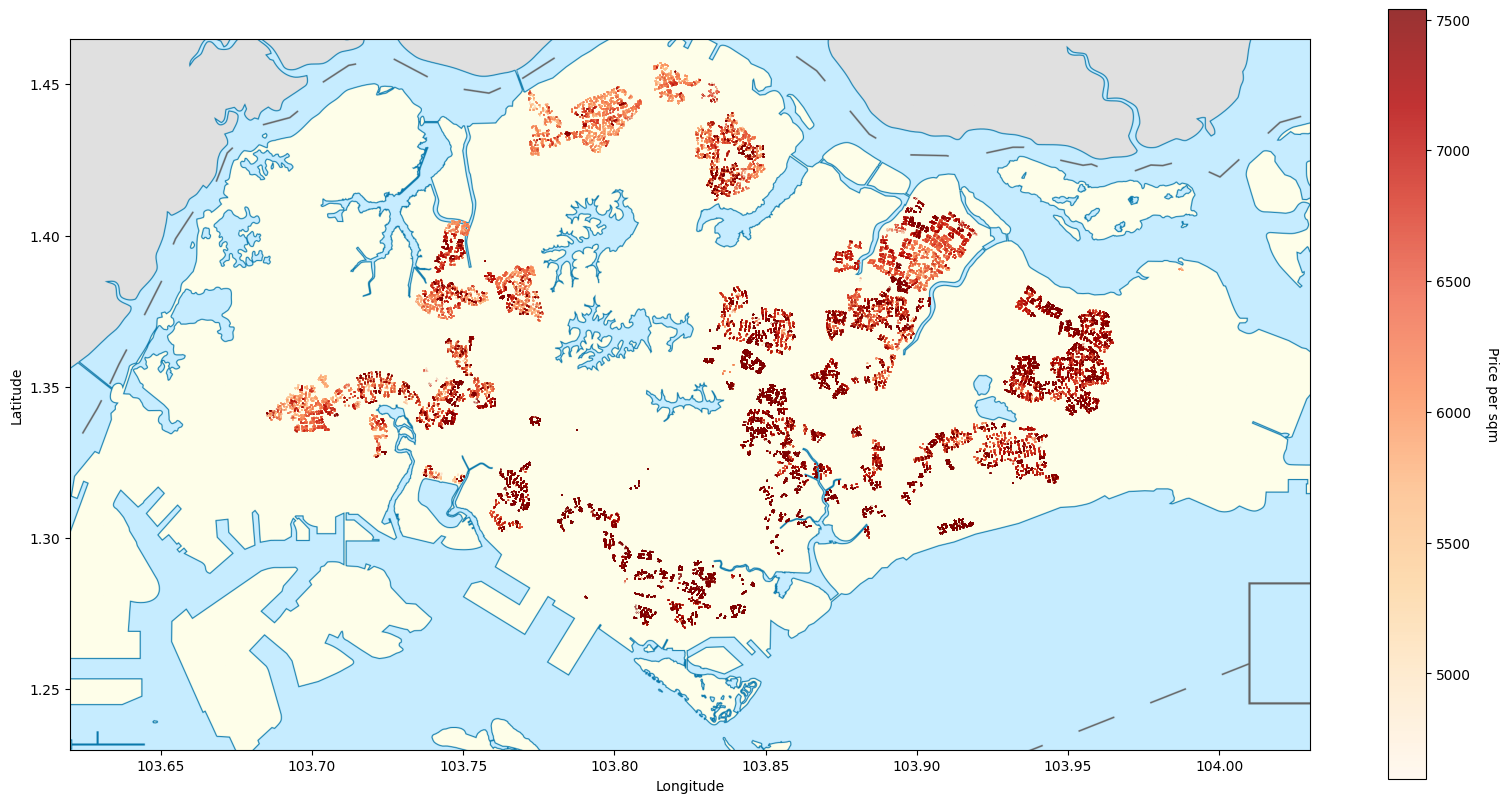
\includegraphics[width=\linewidth]{price_geography.png}
    \caption{Inflation-Adjusted Resale Price per Sqm w.r.t Location}
    \label{fig:price_geography}
\end{figure}

Each transaction contains 3 attributes about the flat's location - town, block and street name. Although these could be seen as categorical data, as there is no meaningful order in the different block numbers or avenues, using one-hot encoding or similar would lead to an even higher dataset dimensionality due to the number of unique values.  
For meaningful analysis, this information is standardised and geocoded into its coordinates - longitude and latitude.

The geocoding process was carried out by joining the block and street address into a single column and then exporting the unique set of addresses within the column into a CSV file. Each address was then fed into the OneMap API (OneMap is a government-produced map developed by the Singapore Land Authority) using a JavaScript program that took in the CSV file. Each API query returns a block's coordinates from the given address query, e.g. \texttt{440B BT BATOK WEST AVE 8} returns \texttt{Long.:103.738218, Lat:1.355138}. This data was then joined to the original dataframe table.


The coordinate data alongside the adjusted price data is visualised in Figure \ref{fig:price_geography}. It can be observed that generally, properties further away from the central business district (southern part of main island) have lower prices, while the high price hotspots tend to be closer. 
Based on this observation, an additional attribute (\texttt{distance\_from\_cbd}) was added that contained the distance between the given flat and the Downtown Core planning area ($1^\circ 17'12''$N, $103^\circ51'13''$E) as calculated using the Haversine formula.


This visualisation also shows the effect that the different towns can have on price as those in the east are more expensive than those in the west as they are more developed and have better transport links, while towns in the north are generally cheaper and more affordable. 
Based on this observation, another categorical attribute is added using one-hot encoding specifying the region the flat is located in.

\section{Splitting Data For Train, Test \& Validation}
The data is first split with 20\% allocated for held-out training data that will be used to evaluate the final model's performance after hyper-parameter tuning and model selection. 
By using the resale price index, the data is now no longer a time series, and hence can be split at random choices without causing data leakage as there no longer exists a temporal relationship between the different transactions. 

As the dataset is large, it is not necessary to do k-fold cross validation, and the rest of the data can just be split 80:20 again for training data and test data that is used to evaluate model performance during training. 
This leaves 562517 samples for training, 140630 for validation, and 175787 samples for held out testing.

\section{General Model Comparison}
The approach taken for model design was to first select a specific model based on a simple testing of the performance without significant hyper-parameter tuning. This section presents the different algorithms tested and their results, while the following section details the hyper-parameter tuning for the best performing model. 

\subsection{Baseline Prediction Algorithm}
To assess the relative performance of regression models, a baseline algorithm was employed to set error metrics that could be used to compare metrics such as mean absolute error (MAE) and root mean-squared error (RMSE). The algorithm generated predictions based soley on the training dataset mean, without consideration of the actual input variables or feature. 
$$y_{\text{predict}} = \overline{y_\text{train}}$$

This naive model had a MAE of \$172,921 and a RMSE of \$223,880, showing that as expected this approach had little to no meaning, given that the dataset mean was \$578,754.

\subsection{Linear Regression}
$$y = \beta_0 + \beta_1 x_1 + ... + \beta_n x_n$$
Linear regression was used first as a model to set a baseline regression accuracy for comparison with other models. 
This approach fits the above equation with coefficients $\beta$ to minimise the residual sum of squares between the response and explanatory variables.

When testing on the validation set, this model had a RMSE of \$92,194 and a MAE of \$69,103, indicating that the predicted prices deviated from the actual prices by those amounts, while the mean absolute percentage error (MAPE)  was 13.46\%. 

While the percentage error may be considered to be reasonable, and there is a huge reduction in error compared to the naive approach, the RMSE and MAE metrics indicate that there still remains a large variance in each prediction from the actual price of the resale flat.
This shows that there is room for improvement by tuning a more refined model.

\subsection{Ridge Regression}
An improvement that can be made to linear regression is to introduce regularisation to prevent over fitting on the training dataset. 
Ridge regression does this by modifying the loss function from simple linear regression to:
$$\text{Loss} = \sum_i (\text{Actual} - \text{Predicted})^2 + \alpha \sum_{i \geq 1}\beta_i^2$$
Parameter $\alpha$ controls the penalty amount, to balance fit and complexity.
Different $\alpha$ values ranging from 1 to 100000 were tested to see the effect of different amounts of regularisation. But they did not show a meaningful improvement over simple linear regression with similar MAE and RMSE values. All $\alpha$ values performed worse than simple linear regression, and large $\alpha$ values such as 10000 led to a significant increase in error.
It was thought that this could have been due to the lack of normalisation of numerical features in the dataset, but this proved not to be the case as similar behaviour was observed after numerical data normalisation.

\subsection{Decision Tree}
A decision tree was also fitted as it takes a different approach to regression as compared to linear regression and ridge regression to evaluate its potential suitability. The decision tree algorithm recursively splits training data based on the most significant input variable at each node, and a prediction is made by traversing the tree and returning the mean or median of samples at the node. 


Without tuning any hyper-parameters, this model had a RMSE value of \$59,269 and a MAE value of \$38,417 which was significantly lower than the previous two approaches. This was demonstrated by the MAPE as well which was 6.91\%.

The trained tree had a depth of 63 which potentially could be pruned to improve model generalisation and hence reduce regression error.

\subsection{K-Nearest Neighbours}
This non-parametric algorithm is instance-based and calculates the weighted average of the k-nearest training examples to predict the value of an unseen observation. k is a hyperparameter and can be adjusted to take more or less observations into account when predicting on unseen data.

After training with 5 nearest neighbours, testing on the validation set gave a RMSE that was \$59,447, MAE was \$38,523 and its MAPE was 6.83\%, showing similar performance to the decision tree.

\subsection{Random Forests}
As it was observed from the previous general tests that the non-parametric algorithms such as the decision tree and K-nearest neighbours had better performance than the parametric linear regression algorithms, research was done into other similar algorithms that would be able to similarly pick up the complex non-linear relationship between the factors and the resale price.

One such algorithm is known as \textit{random forest}, an ensemble algorithm that fits multiple decision trees on the random subsets of the dataset and combines their predictions by averaging. Such an ensemble algorithm can help to prevent overfitting to training data that can occur in simple decision tree regression. 

The algorithm takes samples from the training set and trains decision trees on them, repeatedly until the hyperparameter for number of trees in forest is met.
When doing a prediction, the output of all the decision trees are then taken and averaged to produce a regression prediction.

With the default parameters(100 trees in forest, squared-error for the split quality criterion and no pruning), the random forest regressor achieved a RMSE of \$45,740, MAE of \$30,038 and a MAPE of 5.47\%. 
These error metrics are a lot lower than the decision tree and k-nearest neighbours, which is why the decision was made to optimise the hyperparameters for this particular algorithm as it was thought that it would have the best chance of success. 

\section{Random Forest Hyperparameter Tuning}
Attempts were made to use GridSearchCV to find the best combination of hyperparameters but due to the large dataset and model size, this proved to be infeasible with the given computing resources, therefore a systematic approach where only one hyperparameter was modified at a time was taken.
During hyperparameter tuning, the previously split training and validation data were combined and resplit to prevent overfitting on a single set of validation data. 
This approach takes the aspects of cross-validation to prevent overfitting without the additional calculations as the training dataset is large enough. 

\vspace{-1em}

\begin{figure}[H]
    \centering
    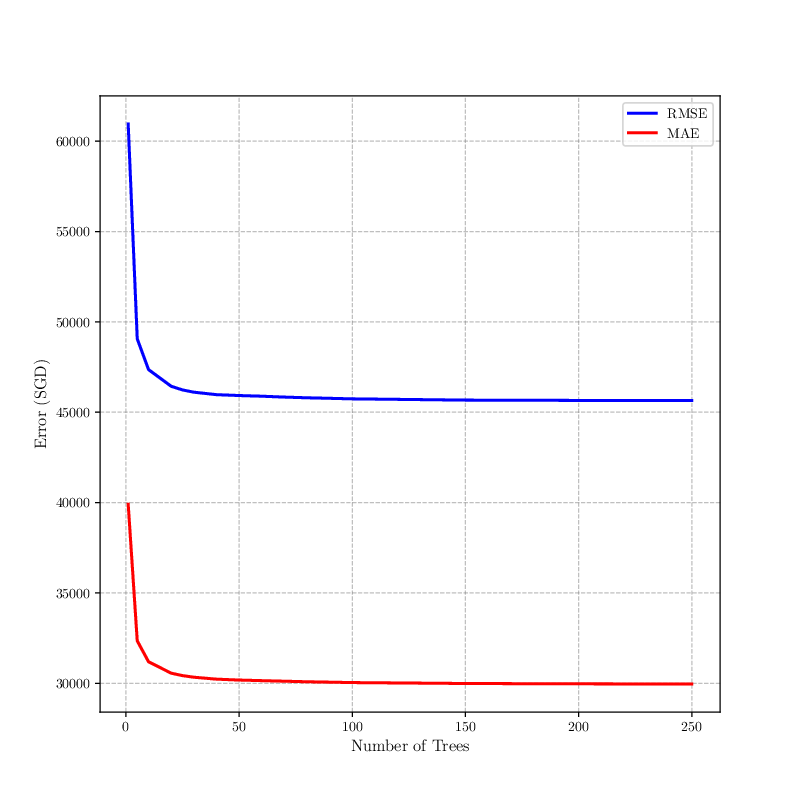
\includegraphics[width=0.85\linewidth]{4_random_forest_hyperparameter_tuning.png}
    \caption{Hyperparameter Tuning: Number of Trees vs Error}
    \label{fig:number-of-trees}
\end{figure}

\subsection{Number of Trees \textit{(Number of Estimators)}}
Random forests average multiple decision trees, and the number of trees used by the algorithm is a hyperparameter that can be adjusted to balance the model's bias-variance trade-off. A high number of trees can result in overfitting, while a low number can lead to high prediction error. Therefore, choosing an optimal number of trees in the forest is critical for achieving good generalization performance.
The training time for a random forest also increases with the number of trees. Therefore, cross-validation was not used due to the large amount of time needed to determine an optimal value. Different values were tested between 1 to 250, and the resulting RMSE of each regressor is plotted alongside the hyperparameter in Figure \ref{fig:number-of-trees}. Values beyond 250 led to application crashes both locally and on Google Colab.


It can be observed from the figure that increasing the number of estimators in the ensemble beyond 75 show minor improvements in actual performance. 

\subsection{Maximum Tree Depth}
The maximum tree depth parameter determines the complexity of the decision trees in the ensemble. A lower maximum tree depth results in simpler trees with reduced variance and increased bias, thus potentially reducing the chance of overfitting but also at the same time increasing the chance that the trees will not be able to capture the relation between the dependent and target variables.

The initial random forest model obtained in section 7 had a maximum tree depth of 65 (the deepest tree in the forest's depth). Therefore, testing was performed with 75 trees and a range of maximum depths between 1 and 70 (representing no pruning). The results are shown in Figure \ref{fig:max-tree-depth}.

\begin{figure}[H]
    \centering
    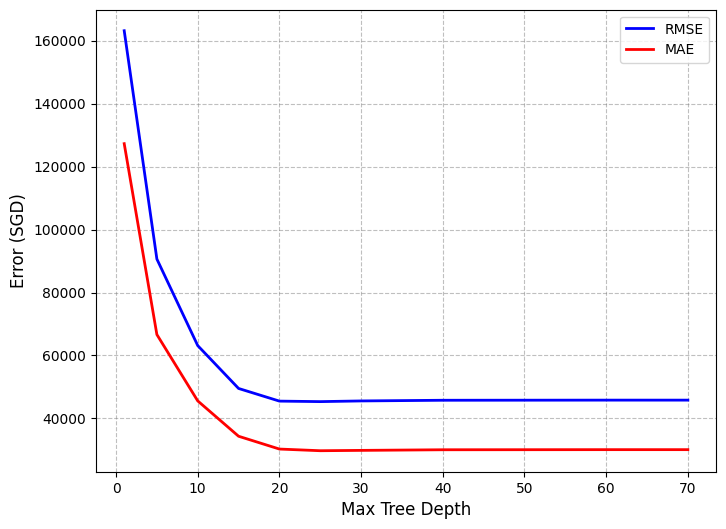
\includegraphics[width=0.85\linewidth]{4_random_forest_max_tree_depth.png}
    \caption{Hyperparameter Tuning: Number of Trees vs Error}
    \label{fig:max-tree-depth}
\end{figure}

Unlike the nuber of estimators hyperparameter where increasing the number of trees continues to reduce error, this hyperparameter had a minimum error point when the maximum tree depth was set at 25. The MAE at this point was \$45,350 and the RMSE was \$29,757.

\subsection{Chosen Hyperparameters}
Based on these two experiments, the number of trees for the random forest was set at 75 and the maximum depth for individual trees was set at 25. 


\section{Evaluation}

\begin{figure}[H]
    \centering
    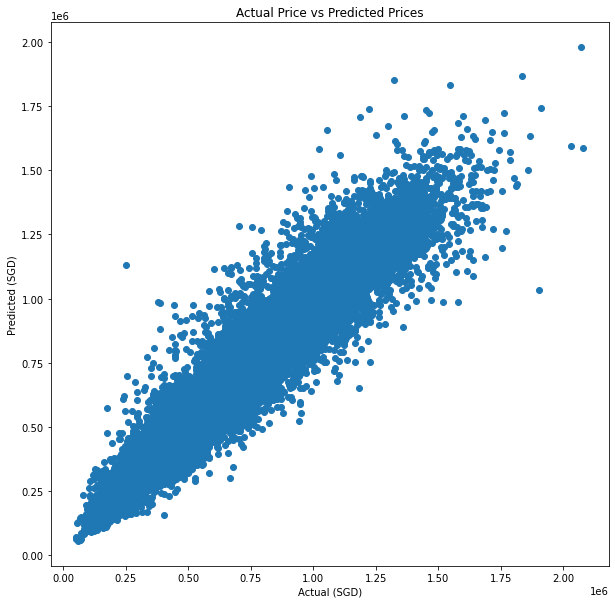
\includegraphics[width=0.75\linewidth]{actual-predicted.png}
    \caption{Predicted Prices vs Actual 
Prices}
    \label{fig:evaluation}
\end{figure}

\subsection{Results}

The model was trained on the combination of the test set and the validation set and tested on the unseen test data to determine the effectiveness of the model. 

The model's performance was similar to results obtained during the previous training process as shown in the table below. Figure \ref{fig:evaluation} also show that for most transactions, the model has a strong prediction that is not far from the actual value. 

\begin{table}[H]
\label{tab:evaluation}
\centering
\begin{tabular}{c|c}
Metric & Value \\\hline
RMSE & SG\$ 45,350 \\
MAE &  SG\$ 29,427 \\
MAPE & 5.35\%
\end{tabular}
\end{table}




\subsection{Potential Error Causes}

\subsubsection{House Price Normalisation}
The choice to use the housing index to normalise the price to the value of the Singaporean dollar in 2023 is an obvious place where error may be introduced into the model.
Certain properties may not have changed in value as much as the adjustment suggests it should have, with certain properties potentially being undervalued after this normalisation and others overvalued. 
There are also factors that may cause a house to be valued differently at two points in time, irrespective of remaining lease length. An example could be that a new MRT station is built close to the property which would not have been accounted for in a sale 20 years ago. 
Such an improvement would lead to the cost of the property increasing, and as the normalisation was done on a country basis rather than a town/street basis, such factors would not be accounted for. 

\subsubsection{Other Unaccounted Factors}
Although there was an attempt to code in geographical data into the model, this model still does not consider other geographical factors such as nearby amenities, supermarkets, or the distance to the bus stop or MRT station. These are generally considered to be valuable to home buyers and can thus influence its pricing.

\subsubsection{High Dataset Dimensionality}
The dataset after preprocessing had 60 different columns due to the one-hot encoding required for the town, region and flat model categories. This may have been a cause of noise in the dataset and may explain why the non-parametric models outperformed linear regression style models. 

\subsubsection{Large Dataset}
The dataset selected also might have been too large. As the data spans a time period of 33 years, it is also possible that limiting the data to recent purchases could have reduced prediction error. 
This would also have reduced training time and enable more hyperparameter testing and tuning.


\subsection{Future Improvements}

\subsubsection{Further Hyperparameter Tuning}
With more time, it would have been interesting to observe if performance could be improved by tuning the other hyperparameters that affect the decision trees created by the random forest algorithm. 

\subsubsection{Alternative Algorithms}Additionally, it is possible that other similar algorithms with improvements such as gradient boosting could outperform the random forest algorithm. Examples include gradient boosted regression trees and Adaboost.

\subsubsection{Individualised Modelling} 
Another potential way of improving performance is to train multiple models based on subsets of the data and combine them together so that the model does not need to generalise as much and spend time trying to find patterns. 
An example could be splitting the dataset into multiple subsets separated by town or by flat type and building individualised models that target a specific town or type.



\end{document}
